%%%%%%%%%%%%%%%%%%%%%%%%%%%%%%%%%%%%%%%%%
% Uppsala University Assignment Title Page 
% LaTeX Template
% Version 1.0 (27/12/12)
%
% This template has been downloaded from:
% http://www.LaTeXTemplates.com
%
% Original author:
% WikiBooks (http://en.wikibooks.org/wiki/LaTeX/Title_Creation)
% Modified by Elsa Slattegard to fit Uppsala university
% License:
% CC BY-NC-SA 3.0 (http://creativecommons.org/licenses/by-nc-sa/3.0/)

%\title{Title page with logo}
%----------------------------------------------------------------------------------------
%	PACKAGES AND OTHER DOCUMENT CONFIGURATIONS
%----------------------------------------------------------------------------------------

\documentclass[12pt]{article}

\usepackage{tikz,lipsum,lmodern}
\usepackage[most]{tcolorbox}

%\usepackage[utf8]{inputenc}
\usepackage[LGR, T1]{fontenc}
\usepackage[greek,english]{babel}
\usepackage{alphabeta}
\usepackage{amsmath}
\usepackage{gfsartemisia}
\usepackage{graphicx}
\usepackage{subfig}
\usepackage{float}
\usepackage[colorinlistoftodos]{todonotes}
\usepackage{tabularx}
\usepackage[myheadings]{fullpage}
\usepackage{enumitem}
\PassOptionsToPackage{hyphens}{url}\usepackage{hyperref}
\usepackage{tikz}
\usepackage[nottoc]{tocbibind} %Adds "References" to the table of contents
\usepackage{xcolor} % to access the named colour LightGray
\definecolor{LightGray}{gray}{0.9}


\usepackage{tabto}
\usepackage{minted}


\usepackage{geometry}
\geometry{
	a4paper,
	total={170mm,257mm},
	left=20mm,
	top=20mm,
}


\addto\captionsenglish{% Replace "english" with the language you use
	\renewcommand{\contentsname}%
	{Περιεχόμενα}%
}

\addto\captionsenglish{
	\renewcommand{\partname}{}
}
\renewcommand{\thepart}{}

\makeatletter
\renewcommand{\fnum@figure}{Εικόνα \thefigure}
\makeatother


\renewcommand{\H}{\textlozenge}

%=====fonts==========%
%\usepackage{libertine}


%====================%





%=============header + footer ======================%
%

\usepackage{fancyhdr}

\pagestyle{fancy}
\fancyhf{}
\rhead{Τεχνολογίες Ανάπτυξης Ηλεκτρονικών Παιχνιδιών 
\includegraphics[width=0.7cm]{UNIPI_(logo).png}}
\lhead{Πανεπιστήμιο Πειραιώς \\ Τμήμα Πληροφορικής}
\cfoot{Σελίδα \thepage}

% 

%\setlength\headheight{47pt}
%=====================================================%



%\setcounter{secnumdepth}{0} % sections are level 1

\begin{document}
	
	\begin{titlepage}
		
		\newcommand{\HRule}{\rule{\linewidth}{0.5mm}} % Defines a new command for the horizontal lines, change thickness here
		
		\center % Center everything on the page
		
		%----------------------------------------------------------------------------------------
		%	HEADING SECTIONS
		%----------------------------------------------------------------------------------------
		
		\textsc{\LARGE Πανεπιστήμιο Πειραιώς}\\[1.5cm] % Name of your university/college
		
\includegraphics[scale=0.6]{UNIPI_(logo).png}\\[1cm] % Include a department/university logo - this will require the graphicx package
		\textsc{\Large Τμήμα Πληροφορικής}\\[0.5cm] % Major heading such as course name
		\textsc{\large Τεχνολογίες Ανάπτυξης Ηλεκτρονικών Παιχνιδιών}\\[0.5cm] % Minor heading such as course title
		
		%----------------------------------------------------------------------------------------
		%	TITLE SECTION
		%----------------------------------------------------------------------------------------
		
		\HRule \\[0.4cm]
		\textsc{\Large Ανάπτυξη 2d παιχνιδιού με SFML \\-\\ Creating a 2d game with SFML\\[0.4cm]} % Minor heading such as course title % Title of your document
		\HRule \\[1.5cm]
		
		%----------------------------------------------------------------------------------------
		%	AUTHOR SECTION
		%----------------------------------------------------------------------------------------
		%
		
		{  \bfseries ΌΝΟΜΑ: Αριστοτέλης Ματακιάς - Α.Μ: Π19100\\[0.4cm] Email Επικοινωνίας: mataktelis01@gmail.com\\[0.4cm] Επιβλέπων καθηγητής: Θεμιστοκλής Παναγιωτόπουλος\\[0.4cm] Ιανουάριος 2023}% Title of your document
		
		
		% If you don't want a supervisor, uncomment the two lines below and remove the section above
		%\Large \emph{Author:}\\
		%John \textsc{Smith}\\[3cm] % Your name
		
		%----------------------------------------------------------------------------------------
		%	DATE SECTION
		%----------------------------------------------------------------------------------------
		
		
		
		\vfill % Fill the rest of the page with whitespace
		
	\end{titlepage}
	
	
	
	%\selectlanguage{greek}
	\tableofcontents
	%\selectlanguage{english}
	
	\newpage

	\section{Εισαγωγή}

	Το παρόν αρχείο αποτελεί την τεκμηρίωση για την εργασία του μαθήματος \textbf{Τεχνολογίες Ανάπτυξης Ηλεκτρονικών Παιχνιδιών}. Στόχος της εργασίας είναι η ανάπτυξη ενός βιντεοπαιχνιδιού. Η γλώσσα προγραμματισμού που επιλέχθηκε είναι η \textbf{C++}. Περισσότερες λεπτομέριες για την υλοποίηση θα παρουσιαστούν σε επόμενες ενότητες.
	
	Ο λόγος για τον οποίο δεν χρησιμοποιήθηκαν τα εργαλεία που παρουσιάστηκαν στο μάθημα (C\# και Unity) είναι ότι παρόλο που επιτρέπουν στον χρήστη να δημιουργήσει εύκολα και γρήγορα ένα παιχνίδι, ο χρήστης δεν γνωρίζει ακριβώς πώς το παιχνίδι λειτουργεί. Μηχανές όπως η Unity παρέχουν ένα έτοιμο περιβάλλον ανάπτυξης πάνω στο οποίο ο χρήστης θα αναπτύξει αυτό που θέλει. Το περιβάλλον αυτό διαχειρίζεται όλες τις λειτουργίες του προγράμματος και απαλλάσσει τον χρήστη από πολλές λεπτομέρειες υλοποίησης, οι οποίες για κάποιους θεωρούνται δύσκολες. Αντίθετα όταν ο ίδιος ο χρήστης δημιουργεί το περιβάλλον, κάτι που μπορεί να επιτευχθεί με γλώσσες χαμηλότερου επιπέδου όπως η C και η C++, μπορεί να το προσαρμόσει ακριβώς στις ανάγκες του. Σαφώς αυτό σημαίνει ότι απαιτείται περισσότερος χρόνος για την ανάπτυξη του παιχνιδιού, καθώς πρώτα πρέπει να φτιαχτεί το περιβάλλον, στο οποίο συνήθως αναφερόμαστε ως μηχανή (engine) του παιχνιδιού. Μπορεί η δημιουργία μίας μηχανής από το μηδέν να ακούγεται ως μία δύσκολη και επίπονη δουλεία αλλά στη πραγματικότητα είναι μία αρκετά δημιουργική διαδικασία για κάθε προγραμματιστή που ασχολείται είτε επαγγελματικά είτε ερασιτεχνικά με την ανάπτυξη βιντεοπαιχνιδιών.
	
	Η εργασία εστιάζει κυρίως στην Υλοποίηση του παιχνιδιού, το οποίο είναι 2D. Επιπλέον οι βιβλιοθήκες και τα περιεχόμενα (Assets) του παιχνιδιού είναι όλα δωρεάν. Ο πηγαίος κώδικας του παιχνιδιού βρίσκεται στα παραδοτέα της εργασίας αλλά και στο Github. Είναι σημαντικό να αναφερθεί ότι ο κώδικας του παιχνιδιού βασίστηκε στο βιβλίο \textbf{SFML Game Development By Example} του οποίου ο κώδικας είναι διαθέσιμος και αποτελεί έναν πολύ καλό οδηγό για εισαγωγή στον προγραμματισμό βιντεοπαιχνιδιών. Η εργασία βασίστηκε στο κεφάλαιο 7 του βιβλίου στο οποίο ενώ δεν περιέχονται όλα σχεδιαστικά πρότυπα (design patterns) του βιβλίου, εξακολουθεί να είναι επαρκές για τη δημιουργία ενός ολοκληρωμένου 2D παιχνιδιού.
	
	%Σαφώς δεν σημαίνει αυτό ότι μία έτοιμη μηχανή ανάπτυξης δεν είναι χρήσιμη, απλά περιορίζει σε έναν βαθμό το χρήστη 
	
	\newpage
	
	
	
	\section{Περιγραφή του προβλήματος}
	
	\subsection{Κριτήρια της εκφώνησης}
	
	Σκοπός της εργασίας είναι η δημιουργία ενός βιντεοπαιχνιδιού και δίνονται τα παρακάτω κριτήρια τα οποία θα πρέπει στην ιδανική περίπτωση να πληρούνται:
	
	\begin{itemize}
		\item \textbf{Αληθοφάνεια} Ο χώρος σας θα πρέπει να "πείθει" τον χρήστη, να μη δημιουργεί την εντύπωση πως παραβιάζει τους φυσικούς νόμους και, γενικά, να παρέχει τη ζητούμενη εμπειρία χωρίς να βασίζεται σε σχεδιαστικές ή αισθητικές ακρότητες.
		
		\item \textbf{Περιεχόμενο} Θα χρησιμοποιήσετε περιεχόμενο που θα θυμίζει τον φυσικό, "πραγματικό" κόσμο για το σύνολο του οποίου θα αναφέρετε πηγές (μέσα στον εικονικό κόσμο, χρησιμοποιώντας κατάλληλα μέσα απεικόνισης πληροφορίας).

		\item \textbf{Πληρότητα}  Ο χώρος θα είναι ολοκληρωμένος σαν συστατικό εφαρμογής εικονικής πραγματικότητας: θα εμφανίζεται στο χρήστη ως ένας τρισδιάστατος κόσμος, θα έχει λειτουργικότητα σε διάφορα σημεία ανάλογα με το τι αναπαριστά και το τι εξυπηρετεί, θα εξελίσσεται με το πέρασμα του χρόνου χάρη σε κινούμενα στοιχεία και στοιχεία με λειτουργικότητα, θα έχει φωτισμό και άλλα διακοσμητικά στοιχεία, και γενικά θα παρέχει μία ολοκληρωμένη, πολυτροπική, δυναμική εμπειρία αναπαράστασης χωρίς αδικαιολόγητα κενά και σημεία ασυνέχειας ή ασυνέπειας.
		
		\item \textbf{Σχεδιασμός} Ο σχεδιασμός του χώρου σας θα χαρακτηρίζεται από ακρίβεια και λεπτομέρεια. Η αυξημένη σχεδιαστική/δομική πολυπλοκότητα δεν αποτελεί στοιχείο το οποίο θα αξιολογηθεί απαραίτητα θετικά.
		
		\item \textbf{Αισθητική} Από άποψη αισθητικής, ο χώρος σας θα πρέπει να είναι ευπαρουσίαστος και να μην χαρακτηρίζεται από αισθητικές ακρότητες. Επίσης, θα πρέπει να “προσκαλεί” τον χρήση και να του κεντρίζει την προσοχή.
		
		\item \textbf{Πρωτοτυπία} Η δομή, ο σχεδιασμός, η αισθητική και η λειτουργικότητα του χώρου σας θα αντανακλούν την έκταση στην οποία διερευνήσατε τις σχεδιαστικές δυνατότητες της πλατφόρμας, τις δυνατότητες της οικείας γλώσσας, καθώς και διάφορα σχεδιαστικά πρότυπα και πρακτικές υλοποίησης.
		
		\item \textbf{Χρηστικότητα} Ο χώρος θα προορίζεται για χρήση από ανθρώπους και για την κάλυψη υπαρκτών αναγκών τους. (π.χ. δυνατότητα μετακίνησης και επίσκεψης διαφόρων σημείων του τρισδιάστατου κόσμου)
		
		\item \textbf{Κίνηση (animation)} Η κατασκευή σας θα περιέχει αναπαραστάσεις κινούμενων στοιχείων, ώστε να δημιουργεί στον χρήστη την εντύπωση ότι συμμετέχει σε ένα δυναμικό, εξελισσόμενο με το χρόνο, κόσμο. Τέτοια στοιχεία μπορεί να είναι, για παράδειγμα, "άψυχα" αντικείμενα, αντικείμενα που μετακινούνται σε προκαθορισμένες διαδρομές, ζώα/ρομπότ, κ.ά. Τονίζεται ότι ο όρος κίνηση χρησιμοποιείται εδώ όχι με την έννοια της μετακίνησης, αλλά της οποιασδήποτε μεταβολής της τιμής κάποιου χαρακτηριστικού ενός αντικειμένου. Έτσι, ως κινούμενο συστατικό νοείται και ένα αντικείμενο που αλλάζει χρώμα με την πάροδο του χρόνου (π.χ., ένα φανάρι ρύθμισης κυκλοφορίας, κ.ά.), ένα αντικείμενο που αλλάζει διαστάσεις, κ.ά.

		\item \textbf{Λειτουργικότητα (functionality)} Ανάλογα με το τι αναπαριστά, η κατασκευή σας θα περιέχει συστατικά με λειτουργικότητα, δηλαδή, συστατικά πάνω στα οποία θα μπορεί να επιδράσει ο χρήστης ή, γενικότερα, συστατικά τα οποία αντιδρούν με συγκεκριμένο τρόπο σε συγκεκριμένες ενέργειες του χρήστη. Παραδείγματα αντικειμένων με λειτουργικότητα είναι μία πόρτα η οποία
		ανοίγει και κλείνει όταν ο χρήστης επιδρά σε ένα διακόπτη, ένας μηχανισμός που ξεκινά και σταματά όταν ο χρήστης επιδρά σε ένα μοχλό, ένα ρομπότ ή ένας συναγερμός που ενεργοποιείται όταν ο χρήστης πλησιάσει κάποιο σημείο του εικονικού κόσμου ή βρεθεί μέσα
		σε κάποια περιοχή του, ένα ραδιόφωνο του οποίου την ένταση ο χρήστης προσαρμόζει με κάποιο χειριστήριο, μία συσκευή τηλεόρασης την οποία ο χρήστης ενεργοποιεί και απενεργοποιεί, κ.ά.
		
		\item \textbf{Ανάπτυξη} Η λειτουργικότητα των διαφόρων αντικειμένων θα υλοποιηθεί στην οικεία γλώσσα (C\#/Unity 3D). Ο κώδικας που θα συντάξετε θα είναι καλά σχεδιασμένος, θα ενσωματώνει βέλτιστες τεχνικές υλοποίησης, θα είναι ευπαρουσίαστος και, το σημαντικότερο, θα είναι συνολικά, αναλυτικά και κατανοητά σχολιασμένος.
		
		
	\end{itemize}

	\subsection{Παρατηρήσεις}
	Το παιχνίδι που θα παρουσιαστεί θα είναι δισδιάστατο (2D) και όχι τρισδιάστατο (3D) όπως αναφέρεται στα κριτήρια, χωρίς να σημαίνει αυτό ότι τα κριτήρια αλλάζουν σημαντικά. Πιο συγκεκριμένα το παιχνίδι θα είναι ένα απλό 2D platformer συγκρίσιμο σε μεγάλο βαθμό με το κλασσικό παιχνίδι \textbf{Super Mario Bros.} (Εικόνα \ref{fig:mario}).
	

 	\begin{figure}[H]
	\centering
	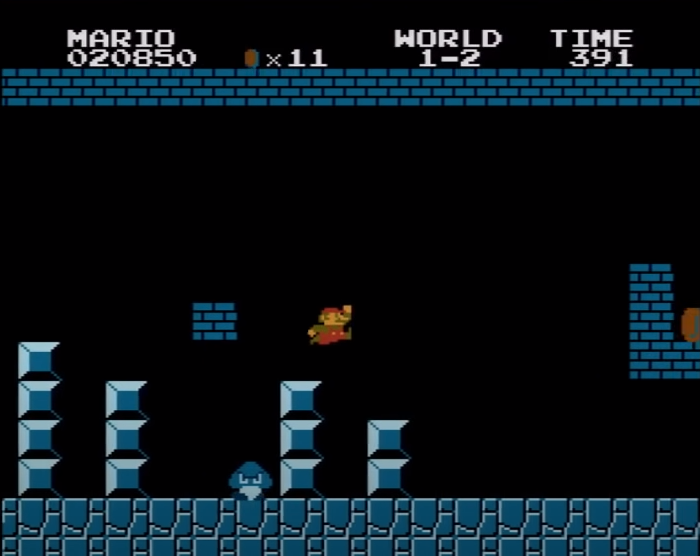
\includegraphics[width=0.65\textwidth]{mario.png}
	\caption{Super Mario Bros. (NES)}
	\label{fig:mario}
	\end{figure}
	
	Ο παίκτης θα μετακινεί με τα τυπικά πλήκτρα \textbf{W}, \textbf{A}, \textbf{S}, \textbf{D} έναν χαρακτήρα σε ένα περιβάλλον φτιαγμένο από \textbf{tiles}. Στο περιβάλλον αυτό θα υπάρχουν "εχθροί" τους οποίους θα μπορεί ο παίκτης να προσπερνά ή να πολεμάει. Σκοπός του παίκτη είναι να φτάσει στο τέλους του χάρτη.

	
	\section{Ανάλυση}
	
	
	Στα πλαίσια της εργασίας είχαν οριστεί οι παρακάτω στόχοι:
	
	\begin{itemize}
		\item \textbf{Χρήση δωρέαν και Open Source περιβάλλοντος για την ανάπτυξη του παιχνιδιού}\\
		Η γλώσσα προγραμματισμού είναι η \textbf{C++} και βασικό ρόλο στην ανάπτυξη του παιχνιδιού έπαιξε η βιβλιοθήκη \textbf{SFML}. Τα αρχικά σημαίνουν \textbf{Simple and Fast Multimedia Library} και είναι μια cross-platform βιβλιοθήκη που παρέχει απλά API για τη δημιουργία παιχνιδιών και εφαρμογών. Η SFML μπορεί να χρησιμοποιηθεί τόσο για την ανάπτυξη μεγάλης κλίμακας εμπορικών παιχνιδιών, όσο και για μικρότερες ομάδες και χομπίστες που είναι αρχάριοι με την C++.
		
		\item \textbf{Χρήση από δωρεάν assets}\\
		Τα assets είναι ένας ευρύς όρος που χρησιμοποιείται για να περιγράψει κάθε μεμονωμένο στοιχείο που υπάρχει σε ένα παιχνίδι. Αυτά μπορεί να περιλαμβάνουν έργα τέχνης, τρισδιάστατα μοντέλα, GUIs, ειδικά, μουσική, ακόμη και scripts για πράγματα όπως η φυσική.
		
		Η δημιουργία game assets αποτελεί ένα έργο σχεδίασης. Ιδανικά, ο δημιουργός ενός παιχνιδιού φτιάχνει ο ίδιος τα assets για το παιχνίδι του, ή στη περίπτωση μίας μεγαλύτερης ομάδας που ασχολείται με την ανάπτυξη ενός παιχνιδιού, θα υπάρχουν άτομα που θα εξειδικεύονται αποκλειστικά σε τέτοια θέματα σχεδίασης. Τα assets είναι αυτά που φαίνονται άμεσα σε αυτόν που βλέπει το παιχνίδι και για πολλούς θεωρείται πώς είναι στοιχειώδης μέρος του ίδιου του παιχνιδιού. 
		
		
		\item \textbf{Δημιουργεία εκτελέσιμου αρχείου για πολλές πλατφόρμες (τουλάχιστον GNU/Linux και Windows)}\\
		
		
		
	\end{itemize}
	
	
	
	
	
	\section{Σχεδίαση}
	
	\section{Υλοποίηση}
	
	\subsection{Προ-επισκόπηση}
	
	Ο πηγαίος κώδικας του προγράμματος αποτελείται από πολλά ξεχωριστά αρχεία. Όπως έχει αναφερθεί στην εισαγωγή, ο κώδικας βασίζεται στον κεφάλαιο 7 του βιβλίου SFML Game development by example. Ο κώδικας του βιβλίου παρέχει μία καλή αρχή για τη δημιουργία ενός παιχνιδιού, έχοντας ορίσει αρκετές βασικές κλάσεις. Ο κώδικας αυτός αξιοποιήθηκε για την δημιουργία ενός πιο ολοκληρωμένου παιχνιδιού. Πιο συγκεκριμένα έγιναν οι παρακάτω προσθήκες:
	
	\begin{itemize}
		\item Προσθήκη ηχητικών εφέ και μουσικής
		
		\item Υλοποίηση ενός απλού συστήματος pick up αντικειμένων για τον παίκτη.
		
		\item Προσθήκη HUD με ενδείξεις healthbar και αντικείμενα που έχουν συλλεχθεί από τον παίκτη
		
		\item Δημιουργία Background Layer στους χάρτες
		
		\item Ορισμός ενός πρακτικού συστήματος για την εύκολη δημιουργία χαρτών
		
		\item Δημιουργία περισσότερων εχθρών
		
		\item Εισαγωγή ενός μεγαλύτερου tileset και αλλαγή του spritesheet για τον παίκτη
		
		\item Διόρθωση διαφόρων bugs στον πρωτογεννή κώδικα
		
		\item Δημιουργία ενός CMakeLists.txt αρχείου (θα εξηγηθεί αναλυτικά σε επόμενη ενότητα)
	\end{itemize}

	Είναι σαφές ότι ο τελικός πηγαίος κώδικας είναι αρκετά μεγάλος και δεν θα εξηγηθεί σε όλη του την έκταση σε αυτό το αρχείο. Αντίθετα έχουν επιλεχθεί κατάλληλα μέρη τα οποία αξίζουν μία επεξήγηση και θα παρουσιαστούν σε επόμενες ενότητες.
	
	Πριν όμως περάσουμε σε εξήγηση του κώδικα πρέπει να αναφερθούμε στην αρχειοθέτηση του project. Ενδεχομένως έμπειροι προγραμματιστές της C++ να έχουν ήδη καταλάβει την αρχειοθέτηση, αλλά για λόγους πληρότητας θα δοθεί μία αναλυτική περιγραφή στην ενότητα που ακολουθεί.
	
	\subsection{Βασικοί ορισμοί και Αρχειοθέτηση του project}
	
	\subsubsection{Header files και Implementation files}
	
	Ο πηγαίος κώδικας του project αποτελείται από πολλές κλάσεις. Είναι σημαντικό να εξηγηθεί πως κάθε κλάση εμφανίζεται στον κώδικα σε δύο αρχεία:
	\begin{itemize}
		\item Το \textbf{header file}, το οποίο έχει κατάληξη \textbf{.h} και περιέχει τον ορισμό (definition) της κλάσης και των συναρτήσεών της.
		
		\item Το αρχείο που περίεχει την υλοποίηση της κλάσης (implementation) και έχει κατάληξη \textbf{.cpp}.
	\end{itemize}
	Με αυτόν τον τρόπο, αν η υλοποίηση μίας κλάσης δεν αλλάξει, δεν χρειάζεται να μεταγλωττιστεί ξανά. Συνήθως τα IDEs θα το κάνουν αυτό αυτόματα, δηλαδή θα μεταγλωττίσουν μόνο τις κλάσεις που έχουν αλλάξει στο πρόγραμμα. Αυτό δεν θα ήταν δυνατό αν για μία κλάση αν αποτελούταν μόνο από ένα αρχείο ή αν υπήρχε υλοποίηση στο header file. Παρακάτω δίνεται ένα απλό παράδειγμα:
	
	\begin{itemize}
		\item Αρχείο \textbf{Num.h}
		
\begin{minted}
[
frame=lines,
framesep=2mm,
baselinestretch=1.1,
bgcolor=LightGray,
fontsize=\footnotesize,
linenos
]{cpp}
class Num {
private:
	int num;
	 
public:
	Num();
	Num(int n);
	int getNum();
}; 
\end{minted}

		\item Αρχείο \textbf{Num.cpp}

\begin{minted}
	[
	frame=lines,
	framesep=2mm,
	baselinestretch=1.1,
	bgcolor=LightGray,
	fontsize=\footnotesize,
	linenos
	]{cpp}
#include "Num.h"

Num::Num() : num(0) { } // constructor definition: 
			// ": num(0)" is the initializer list
			// "{ }" is the function body

Num::Num(int n) : num(n) { } // similarly ": num(n)" is the initializer list

int Num::getNum() {
	return num;
}
\end{minted}


		\item Αρχείο \textbf{main.cpp}

\begin{minted}
	[
	frame=lines,
	framesep=2mm,
	baselinestretch=1.1,
	bgcolor=LightGray,
	fontsize=\footnotesize,
	linenos
	]{cpp}
#include <iostream>
#include "Num.h"

int main()
{
	Num n(35);
	std::cout << n.getNum() << std::endl;
	return 0;
} 
\end{minted}

	\end{itemize}
	
	
	Για να κάνουμε compile αρκεί να δώσουμε στον μεταγλωττιστή g++ τα αρχεία main.cpp και Num.cpp με την παρακάτω εντολή:
	
\begin{minted}{bash}
$ g++ main.cpp Num.cpp
\end{minted}	
	
	
	Όπως βλέπουμε στα παραπάνω αρχεία, κάθε .cpp αρχείο μπορεί να χρησιμοποιήσει ένα header αρχείο μέσω ενός include statement (γραμμή 1 στο Num.cpp και γραμμή 2 στο main.cpp). Γενικά τα header files περιέχουν ορισμούς συναρτήσεων και μέσω της δήλωσης \#include ο μεταγλωττιστής ενημερώνεται πως πρέπει πρώτα να μεταγλωττιστούν οι συναρτήσεις που είναι καταγεγραμμένες στο header file και στη συνέχεια θα μεταγλωττίσει το τωρινό αρχείο.
	
	Υπάρχουν δύο ειδών header files:
	
	\begin{itemize}
		\item \textbf{Standard library header files} (όπως το iostream στη γραμμή 1 του αρχείου \textbf{main.cpp})\\
		Τα αρχεία αυτά περιέχονται ήδη στον g++ μεταγλωττιστή. Παρόμοια βιβλιοθήκες που έχουν εγκατασταθεί, όπως και η SFML μπορούν να κληθούν με τον ίδιο τρόπο εφόσον έχουν οριστεί στο PATH του υπολογιστή.
		
		\item \textbf{User-defined header files} (όπως το Num.h του παραδείγματος)\\
		Αυτά τα header files έχουν δημιουργηθεί από τον χρήστη. Μπορούμε να τα ξεχωρίσουμε καθώς στο include statement το όνομά τους είναι μέσα σε double quotes και όχι μέσα σε "<" και ">".		
	\end{itemize}


	Πριν προχωρήσουμε καλό είναι να επισημάνουμε τα \textbf{initializer list} που αναφέρονται και στα σχόλια του παραδείγματος, καθώς χρησιμοποιούνται αρκετά στον κώδικα του project. Πιο συγκεκριμένα, το \textbf{initializer list} χρησιμοποιείται για να αρχικοποιήσει πεδία μίας κλάσης. Δηλώνεται μετά το όνομα του constructor και των παραμέτρων του. Το \textbf{initializer list} ξεκινάει με τον χαρακτήρα ":" και αποτελείται από μία λίστα μεταβλητών οι οποίες θα αρχικοποιηθούν. Οι μεταβλητές χωρίζονται με κόμμα και οι τιμές των μεταβλητών δίνονται μέσα σε παρενθέσεις. Παρακάτω φαίνεται άλλο ένα παράδειγμα χρήσης των \textbf{initializer list} από τον constructor της κλάσης EntityBase του πηγαίου κώδικα από το παιχνίδι.

\begin{minted}
	[
	frame=lines,
	framesep=2mm,
	baselinestretch=1.1,
	bgcolor=LightGray,
	fontsize=\footnotesize
	]{cpp}
EntityBase::EntityBase(EntityManager* l_entityMgr)
	:m_entityManager(l_entityMgr), m_name("BaseEntity"), 
	m_type(EntityType::Base), m_id(0), m_referenceTile(nullptr),
	m_state(EntityState::Idle), m_collidingOnX(false), m_collidingOnY(false){}
\end{minted}

	Το \textbf{initializer list} βοηθάει ώστε ο κώδικας να είναι πιο περιεκτικός και καθαρός, ειδικά σε περιπτώσεις όπως στο παραπάνω παράδειγμα όπου μόνος σκοπός του constructor είναι οι ανάθεση τιμών σε πεδία της κλάσης.
		
	\subsubsection{Κλήση ενός header file}
	Επιστρέφουμε στο παράδειγμα της κλάσης Num και επισημάνουμε πως η δεν πρέπει στην C++ ένα header file να γίνεται include πολλές φορές. Ωστόσο 
		
		
	
	\subsubsection{Αρχειοθέτηση}
	
	Ο πηγαίος κώδικας βρίσκεται στον φάκελο \textbf{Simple-SFML-2D-Game} και αποτελείται από \textbf{.cpp} αρχεία και \textbf{.h} αρχεία. Τα \textbf{.cpp} αρχεία βρίσκονται στον φάκελο src και τα \textbf{.h} αρχεία στον φάκελο \textbf{include} αντίστοιχα. 
	
	

	
	
	
	
	\subsection{Διαχείριση εισόδου από τον χρήστη}
	
	\subsection{Καταστάσεις του προγράμματος}
	Ένα βιντεοπαιχνίδι δεν αποτελείται μόνο από γραφικά. Είναι πολύ συνηθισμένο σήμερα ένα παιχνίδι να έχει μια εισαγωγή πριν την έναρξή του, η οποία μάλιστα θα συνοδεύεται από κάποιο animation. Επίσης είναι αναγκαίο να ύπαρχει και ένα μενού από το οποίο ο χρήστης θα ξεκινάει το παιχνίδι ή θα επιλέγει ανάμεσα σε ορισμένες ρυθμίσεις ή θα κλείνει την εφαρμογή. Είναι σημαντικό επίσης το παιχνίδι να έχει τη δυνατότητα να διακόπτεται (pause) από τον χρήστη. Όλες αυτές οι λειτουργικότητες πρέπει να ληφθούν υπ'όψη από τα πρώτα στάδια ανάπτυξης ενός παιχνιδιού. Ο τρόπος με τον οποίο θα αντιμετωπιστούν αυτές οι απαιτήσεις είναι μέσω της υλοποίησης των \textbf{καταστάσεων}.
	
	Πριν συνεχίσουμε πρέπει να εξηγηθεί ακριβώς η έννοια της \textbf{κατάστασης} σε ένα παιχνίδι. Πρόκειται για ένα από τα πολλά επίπεδα (layers) που μπορεί να έχει ένα παιχνίδι, όπως το κεντρικό μενού, το animation που εμφανίζεται πριν το κεντρικό μενού και τέλος το ίδιο το παιχνίδι. Κάθε ένα από αυτά τα επίπεδα έχει τον δικό του τρόπο να ενημερώνεται και να κάνει render τα περιεχόμενά του στην οθόνη.
	
	Το βιβλίο SFML Game Development by example προτείνει μία υλοποίηση αρκετά καλή για τα πλαίσια της εργασίας και έχει ενσωματωθεί στον πηγαίο κώδικα. Βασικό στοιχείο της υλοποίησης είναι η \textbf{δημιουργία ξεχωριστών κλάσεων} για τη κάθε κατάσταση. Όλες οι κλάσεις θα έχουν ορισμένες κοινές μεθόδους για να ενημερώνονται και να κάνουν render, κάτι που επιτυχγάνεται με την \textbf{κληρονομικότητα}. Παρακάτω ορίζουμε την κλάση BaseState, από την οποία θα κληρωνομούν όλες οι κλάσεις που αντιστοιχούν σε μία κατάσταση του παιχνιδιού.
	
	
	Επειδή είναι αναγκαίο κάθε κλάση που κληρωνομεί από την BaseState να έχει υλοποιήσει τις μεθόδους της, όλες οι μέθοδοι δηλώνονται ως \textbf{purely virtual} (έχουν το keyword 'virtual' και στο τέλος '=0').
	
	\subsection{Κλάση Map}
	
	\subsection{Δημιουργία Χαρτών}
	
	\subsection{Δημιουργία Εχθρών}
	
	\section{Εκτέλεση}
	
	\section{Κάλυψη κριτηρίων}
	
	\section{Συμπεράσματα και παρατηρήσεις}
	
	\section{Βιβλιογραφία}

	
	
	
\end{document}